% CS765A Advanced Programming in the UNIX Environment
% Author: Jan Schaumann <jschauma@netmeister.org>
% $Id: slides.tex,v 1.6 2005/08/30 21:43:10 jschauma Exp $
%\special{! TeXDict begin /landplus90{true}store end }

\documentclass[sxga]{xdvislides}
\usepackage[landscape]{geometry}
\usepackage{graphics}
\usepackage{graphicx}
\usepackage{colordvi}
\usepackage{alltt}
\usepackage{upquote}

\begin{document}
\setfontphv

%%% Headers and footers
\lhead{\slidetitle}
\chead{CS631 - Advanced Programming in the UNIX Environment}
\rhead{Slide \thepage}
\lfoot{\Gray{Lecture 01: Introduction, UNIX history, UNIX Programming Basics}}
\cfoot{\relax}
\rfoot{\Gray{\today}}

\vspace*{\fill}
\begin{center}
	\Hugesize
		CS631 - Advanced Programming in the UNIX Environment\\ [1em]
	\hspace*{5mm}\blueline\\ [1em]
	\Normalsize
		Department of Computer Science\\
		Stevens Institute of Technology\\
		Jan Schaumann\\
		\verb+jschauma@stevens.edu+\\
		\verb+http://www.cs.stevens.edu/~jschauma/631/+
\end{center}
\vspace*{\fill}

\subsection{New Rules}
\Hugesize
\vspace*{\fill}
\begin{center}
Close your laptops!
\end{center}
\vspace*{\fill}
\Normalsize

\subsection{New Rules}
\Hugesize
\vspace*{\fill}
\begin{center}
Close your laptops! \\
\vspace{.5in}
Open your eyes! \\
\small
(Mind, too.)
\end{center}
\vspace*{\fill}
\Normalsize


\subsection{What is this about?}
\begin{center}
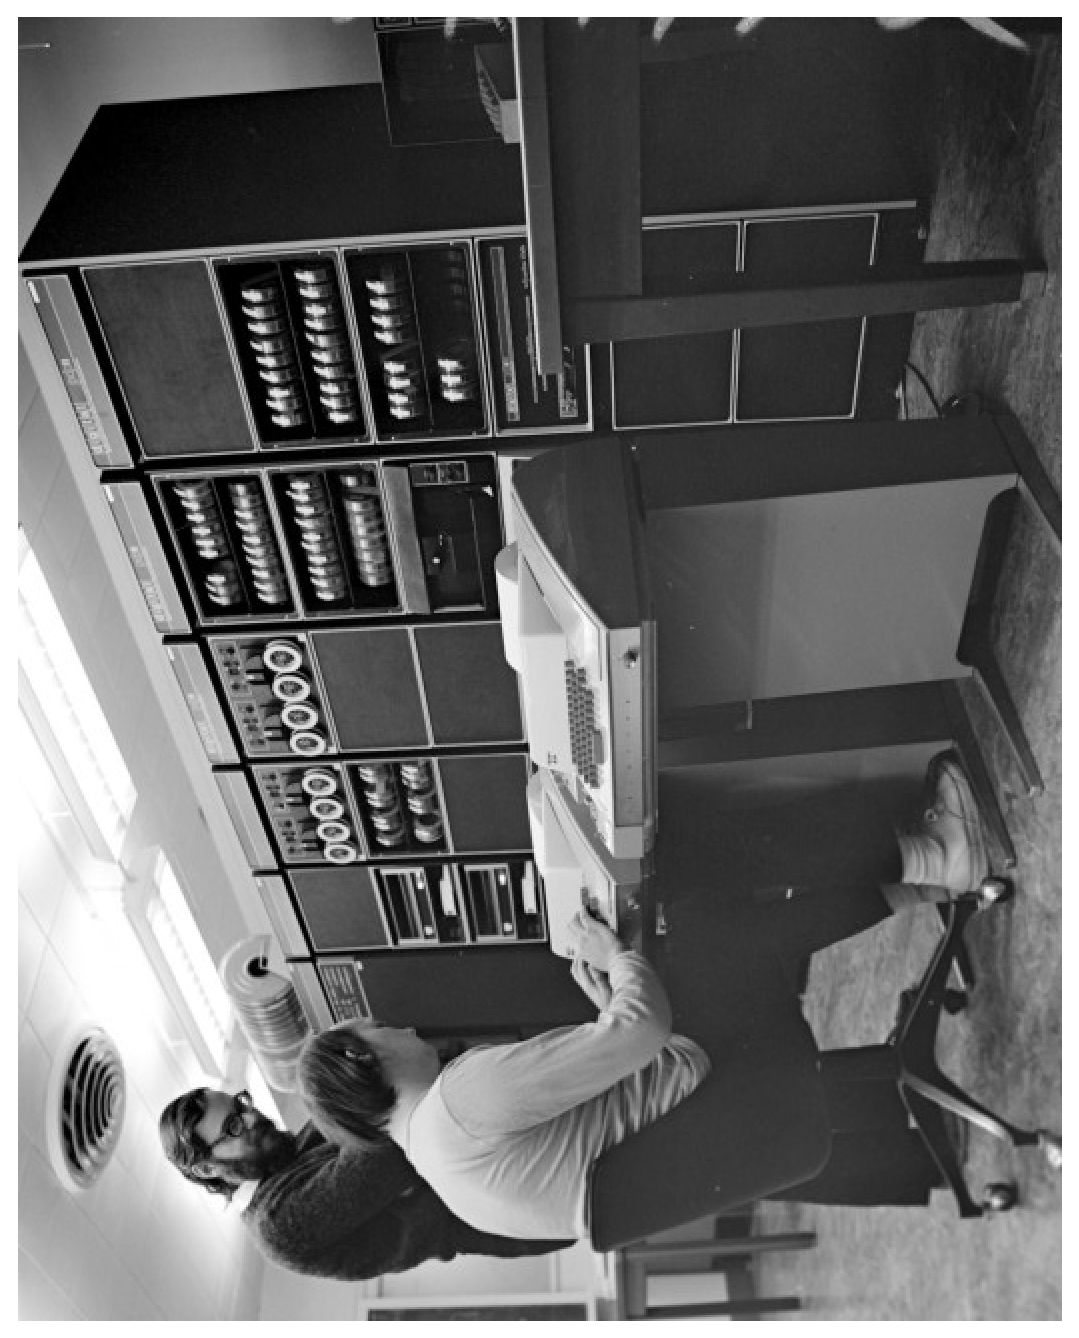
\includegraphics[scale=0.6,angle=-90]{pics/kernighan-ritchie.eps} \\
\verb+http://cm.bell-labs.com/who/dmr/chist.html+
\end{center}

\subsection{In a nutshell: the "what"}
\begin{verbatim}
$ ls /bin
[          csh        ed         ls         pwd        sleep
cat        date       expr       mkdir      rcmd       stty
chio       dd         hostname   mt         rcp        sync
chmod      df         kill       mv         rm         systrace
cp         domainname ksh        pax        rmdir      tar
cpio       echo       ln         ps         sh         test
$
\end{verbatim}

See also:
\begin{verbatim}
$ ssh linux-lab.cs.stevens.edu
$ cd ~jschauma/apue/src/
\end{verbatim}

\subsection{In a nutshell: the "what"}
\begin{verbatim}
$ grep "(int" /usr/include/sys/socket.h
int	accept(int, struct sockaddr * __restrict, socklen_t * __restrict);
int	bind(int, const struct sockaddr *, socklen_t);
int	connect(int, const struct sockaddr *, socklen_t);
int	getsockopt(int, int, int, void * __restrict, socklen_t * __restrict);
int	listen(int, int);
ssize_t	recv(int, void *, size_t, int);
ssize_t	recvfrom(int, void * __restrict, size_t, int,
ssize_t	recvmsg(int, struct msghdr *, int);
ssize_t	send(int, const void *, size_t, int);
ssize_t	sendto(int, const void *,
ssize_t	sendmsg(int, const struct msghdr *, int);
int	setsockopt(int, int, int, const void *, socklen_t);
int	socket(int, int, int);
int	socketpair(int, int, int, int *);
$
\end{verbatim}

\subsection{In a nutshell: the "what"}
\begin{itemize}
	\item gain an understanding of the UNIX operating systems
	\item gain (systems) programming experience
	\item understand fundamental OS concepts (with focus on UNIX family):
		\begin{itemize}
			\item multi-user concepts
			\item basic and advanced I/O
			\item process relationships
			\item interprocess communication
			\item basic network programming using a client/server model
		\end{itemize}
\end{itemize}

\subsection{In a nutshell}
The "why":
\begin{itemize}
	\item understanding how UNIX works gives you insights in other OS concepts
	\item system level programming experience is invaluable as it
		forms the basis for most other programming and even {\em
		use} of the system
	\item system level programming in C helps you understand general
		programming concepts
	\item most higher level programming languages (eventually) call
		(or implement themselves) standard C library functions
\end{itemize}

\subsection{In a nutshell: the "how"}
\small
\begin{verbatim}

    static char dot[] = ".", *dotav[] = { dot, NULL };
    struct winsize win;
    int ch, fts_options;
    int kflag = 0;
    const char *p;

    setprogname(argv[0]);
    setlocale(LC_ALL, "");

    /* Terminal defaults to -Cq, non-terminal defaults to -1. */
    if (isatty(STDOUT_FILENO)) {
        if (ioctl(STDOUT_FILENO, TIOCGWINSZ, &win) == 0 &&
            win.ws_col > 0)
            termwidth = win.ws_col;
        f_column = f_nonprint = 1;
    } else
        f_singlecol = 1;

    /* Root is -A automatically. */
    if (!getuid())
        f_listdot = 1;

    fts_options = FTS_PHYSICAL;
    while ((ch = getopt(argc, argv, "1ABCFLRSTWabcdfghiklmnopqrstuwx")) != -1) {
        switch (ch) {
        /*
         * The -1, -C, -l, -m and -x options all override each other so
         * shell aliasing works correctly.
         */
        case '1':
            f_singlecol = 1;
\end{verbatim}
\Normalsize

\subsection{In a nutshell: the "how"}
\begin{verbatim}
$ $EDITOR cmd.c
$ cc -Wall -g -o cmd cmd.c
$ ./cmd
$ echo "Hooray!"
Hooray!
$
\end{verbatim}

\subsection{In a nutshell: the "how"}
\Hugesize
\vspace*{\fill}
\begin{center}
Open your laptops!
\end{center}
\begin{verbatim}
$ ssh linux-lab.cs.stevens.edu
$ mkdir apue
$ cp ~jschauma/apue/01/welcome.c apue/
\end{verbatim}
\vspace{.5in}
Now compile and run the program.
\vspace*{\fill}
\Normalsize

\subsection{In a nutshell: the "how"}
\begin{verbatim}
$ $EDITOR cmd.c
$ cc -Wall -g -o cmd cmd.c
$ ./cmd
$ echo "Hooray!"
Hooray!
$
\end{verbatim}

\subsection{In a nutshell: the "how"}
\begin{verbatim}
$ $EDITOR cmd.c
$ cc -Wall -g -o cmd cmd.c
cmd.c: In function `main':
cmd.c:19: error: parse error before "return"
$
\end{verbatim}

\subsection{In a nutshell: the "how"}
\begin{verbatim}
$ $EDITOR cmd.c
$ cc -Wall -g -o cmd cmd.c
cmd.c: In function `main':
cmd.c:19: error: parse error before "return"
$ $EDITOR cmd.c
$ cc -Wall -g -o cmd cmd.c
$ ./cmd
Memory fault (core dumped)
$
\end{verbatim}

\subsection{In a nutshell: the "how"}
\begin{verbatim}
$ $EDITOR cmd.c
$ cc -Wall -g -o cmd cmd.c
cmd.c: In function `main':
cmd.c:19: error: parse error before "return"
$ $EDITOR cmd.c
$ cc -Wall -g -o cmd cmd.c
$ ./cmd
Memory fault (core dumped)
$ echo "!@#!@!!!??#@!"
!@#!@!!!??#@!
$ gdb ./cmd cmd.core
Program terminated with signal 11, Segmentation fault.
Loaded symbols for /usr/libexec/ld.elf_so
#0  0xbbbc676a in __findenv () from /usr/lib/libc.so.12
(gdb)
\end{verbatim}

\subsection{Programming}
\begin{center}
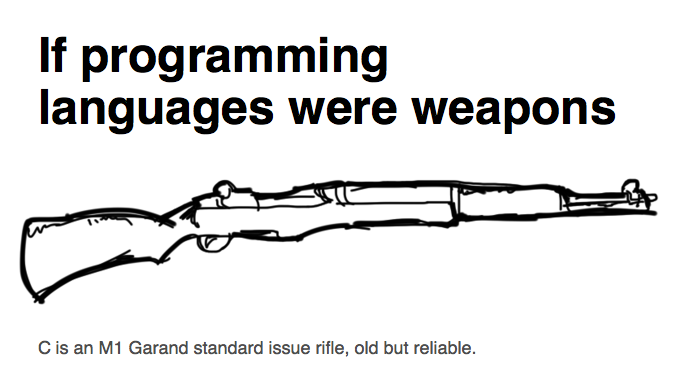
\includegraphics[scale=0.7,angle=-90]{pics/if-programming-languages-were-weapons.eps} \\
\vspace{.5in}
\verb+http://is.gd/6aidgb+ \\
\verb+https://i.imgur.com/ZyeCO.jpg+
\end{center}

\subsection{About this class}
Textbook:
\begin{itemize}
	\item ``Advanced Programming in the UNIX Environment'', by
		W. Richard Stevens, Stephen A. Rago (3rd Edition)
\end{itemize}
\addvspace{.25in}
Help:
\begin{itemize}
	\item \verb+http://lists.stevens.edu/cgi-bin/mailman/listinfo/cs631apue+
	\item IRC: \verb+#cs631apue+ on Freenode
	\item \verb+https://twitter.com/#!/cs631apue+
\end{itemize}
\addvspace{.25in}

Grading:
\begin{itemize}
	\item 5 homework assignments, worth 20 points each
	\item 1 midterm project, worth 100 points
	\item 1 final project (group work), worth 200 points
	\item 1 final programming assignment (individual), worth 100 points
	\item no curve
\end{itemize}

\subsection{Syllabus}
%Topics:
\begin{itemize}
	\item 08/31: Introduction, UNIX history, UNIX Programming Basics
	\item 09/14: File I/O, File Sharing
	\item 09/21: Files and Directories, Filesystems
	\item 09/28: No Class
	\item 10/05: System Data Files, Time \& Date, Process Environment
	\item 10/13: Process Control, Signals
	\item 10/19: Process Groups, Signals
	\item 10/26: Interprocess Communication
	\item 11/02: Advanced I/O: Nonblocking I/O, Polling, and Record Locking
	\item 11/09: Daemon Processes, final project discussion
	\item 11/16: UNIX tools: make(1), gdb(1), revision control, etc.
	\item 11/23: Code reading and discussions
	\item 11/20: Encryption
	\item 12/07: Review
\end{itemize}

\pagebreak

\vspace*{\fill}
\begin{center}
  \Hugesize
    UNIX History
	\hspace*{5mm}\blueline\\ [1em]
  \Normalsize
\end{center}
\vspace*{\fill}

\subsection{UNIX history}
\verb+http://www.unix.org/what_is_unix/history_timeline.html+ \\

\begin{itemize}
	\item Originally developed in 1969 at Bell Labs by Ken Thompson
		and Dennis Ritchie.
	\item 1973, Rewritten in C. This made it portable and changed the history of OS
	\item 1974: Thompson, Joy, Haley and students at Berkeley develop
		the {\bf B}erkeley {\bf S}oftware {\bf D}istribution (BSD) of UNIX
	\item two main directions emerge: BSD and what was to become ``System V''
\end{itemize}

\subsection{Notable dates in UNIX history}
\begin{itemize}
	\item 1984 4.2BSD released (TCP/IP)
	\item 1986 4.3BSD released (NFS)
	\item 1991 Linus Torvalds starts working on the Linux kernel
	\item 1993 Settlement of USL vs. BSDi; NetBSD, then FreeBSD are created
	\item 1994 Single UNIX Specification introduced
	\item 1995 4.4BSD-Lite Release 2 (last CSRG release); OpenBSD
		forked off NetBSD
	\item 2000 Darwin created (derived from NeXT, FreeBSD, NetBSD)
	\item 2003 Xen; SELinux
	\item 2005 Hadoop; DTrace; ZFS; Solaris Containers
	\item 2006 AWS ("Cloud Computing" comes full circle)
	\item 2007 iOS; KVM appears in Linux
	\item 2008 Android; Solaris open sourced as OpenSolaris
\end{itemize}

\subsection{Some UNIX versions}
More UNIX (some generic, some trademark, some just unix-like):
\\

\small
\begin{tabular}{ c c c c c}
	1BSD & 2BSD & 3BSD & 4BSD & 4.4BSD Lite 1 \\
	4.4BSD Lite 2 & 386 BSD & A/UX & Acorn RISC iX & AIX \\
	AIX PS/2 & AIX/370 & AIX/6000 & AIX/ESA & AIX/RT \\
	AMiX & AOS Lite & AOS Reno & ArchBSD & ASV \\
	Atari Unix & BOS & BRL Unix & BSD Net/1 & BSD Net/2 \\
	BSD/386 & BSD/OS & CB Unix & Chorus & Chorus/MiX \\
	Coherent & CTIX & Darwin & Debian GNU/Hurd & DEC OSF/1 ACP \\
	Digital Unix & DragonFly BSD & Dynix & Dynix/ptx & ekkoBSD \\
	FreeBSD & GNU & GNU-Darwin & HPBSD & HP-UX \\
	HP-UX BLS & IBM AOS & IBM IX/370 & Interactive 386/ix & Interactive IS \\
	IRIX & Linux & Lites & LSX & Mac OS X \\
	Mac OS X Server & Mach & MERT & MicroBSD & Mini Unix \\
	Minix & Minix-VMD & MIPS OS & MirBSD & Mk Linux \\
	Monterey & more/BSD & mt Xinu & MVS/ESA OpenEdition & NetBSD \\
	NeXTSTEP & NonStop-UX & Open Desktop & Open UNIX & OpenBSD \\
	OpenServer & OPENSTEP & OS/390 OpenEdition & OS/390 Unix & OSF/1 \\
	PC/IX & Plan 9 & PWB & PWB/UNIX & QNX \\
	QNX RTOS & QNX/Neutrino & QUNIX & ReliantUnix & Rhapsody \\
	RISC iX & RT & SCO UNIX & SCO UnixWare & SCO Xenix \\
	SCO Xenix System V/386 & Security-Enhanced Linux & Sinix &
		Sinix ReliantUnix & Solaris \\
	SPIX & SunOS & Tru64 Unix & Trusted IRIX/B & Trusted Solaris \\
	Trusted Xenix & TS & UCLA Locus & UCLA Secure Unix & Ultrix \\
	Ultrix 32M & Ultrix-11 & Unicos & Unicos/mk & Unicox-max \\
	UNICS & UNIX 32V & UNIX Interactive & UNIX System III & UNIX System IV \\
	UNIX System V & UNIX System V Release 2 & UNIX System V Release 3 &
		UNIX System V Release 4 & UNIX System V/286 \\
	UNIX System V/386 & UNIX Time-Sharing System & UnixWare & UNSW & USG \\
	Venix & Wollogong & Xenix OS & Xinu & xMach \\
\end{tabular}
\Normalsize

\subsection{UNIX Timeline}
\Hugesize
\vspace*{\fill}
\begin{center}
\begin{verbatim}
unix.png  : http://www.levenez.com/unix/
linux.png : http://futurist.se/gldt/
\end{verbatim}
\end{center}
\vspace*{\fill}
\Normalsize



\subsection{UNIX Everywhere}
\Hugesize
\vspace*{\fill}
\begin{center}
Today, your desktop, server, cloud, TV, phone, watch, stereo, car
navigation system, thermostat, door lock, etc. all run a Unix-like OS... \\
\end{center}
\vspace*{\fill}
\Normalsize

\subsection{UNIX Everywhere}
\Hugesize
\vspace*{\fill}
\begin{center}
Today, your desktop, server, cloud, TV, phone, watch, stereo, car
navigation system, thermostat, door lock, etc. all run a Unix-like OS... \\
\vspace{.5in}
...with all the risks that entails.
\end{center}
\vspace*{\fill}
\Normalsize

\pagebreak

\vspace*{\fill}
\begin{center}
  \Hugesize
    UNIX Basics
	\hspace*{5mm}\blueline\\ [1em]
  \Normalsize
\end{center}
\vspace*{\fill}

\subsection{UNIX Basics: Architecture}
\begin{center}
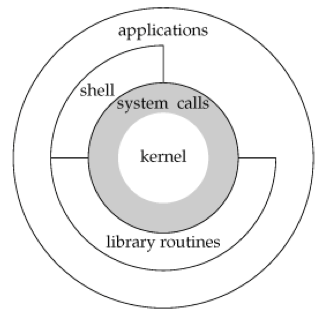
\includegraphics[angle=-90]{pics/unix_architecture.eps}
\end{center}

\subsection{System Calls and Library Functions, Standards}
{\bf System Calls and Library Functions}
\begin{itemize}
	\item {\em System calls} are entry points into kernel code where their functions
		are implemented.  Documented in section 2 of the manual (e.g. {\tt
		write(2)}).
	\item {\em Library calls} are transfers to user code which performs the desired
		functions. Documented in section 3 of the manual (e.g. {\tt
		printf(3)}).
\end{itemize}
\vspace{.5in}
{\bf Standards}
\begin{itemize}
	\item ANSI C (X3.159-1989) C89, C9X/C99 (ISO/IEC 9899), C11 (ISO/IEC 9899:2011)
	\item IEEE POSIX (1003.1-2008) / SUSv4
\end{itemize}

\subsection{Important ANSI C Features, Error Handling}
\begin{itemize}
	\item	Important ANSI C Features:
		\begin{itemize}
			\item function prototypes
			\item generic pointers ({\tt void *})
			\item abstract data types (e.g. {\tt pid\_t}, {\tt size\_t})
		\end{itemize}
	\item	Error Handling:
		\begin{itemize}
			\item meaningful return values
			\item {\tt errno} variable
			\item look up constant error values via two functions:
				\small
				\setlength{\unitlength}{1mm}
				\begin{center}
					\begin{picture}(200,20)
						\thinlines
						\put(-10,0){\framebox(180,15){}}
						\put(0,10){{\tt \#include <string.h>}}
						\put(0,5){{\tt char *strerror(int {\em errnum})}}
						\put(100,2){Returns: pointer to message string}
					\end{picture}
					\begin{picture}(200,20)
						\thinlines
						\put(-10,0){\framebox(180,15){}}
						\put(0,10){{\tt \#include <stdio.h>}}
						\put(0,5){{\tt void perror(const char {\em *msg})}}
					\end{picture}
				\end{center}
		\end{itemize}
\end{itemize}

\subsection{UNIX Basics: Pipelines}
What is the longest word found on the ten most
frequently retrieved English Wikipedia pages?
\begin{verbatim}
for f in $(curl -L http://is.gd/c6F2fs | zgrep -i "^en " |
        sort -k3 -n | tail -10 |
        sed -e 's/en \(.*\) [0-9]* [0-9]*/\1/'); do
        links -dump http://en.wikipedia.org/wiki/${f}
done |
tr '[:punct:]' ' ' |
tr '[:space:]' '\n' |
tr '[:upper:]' '[:lower:]' |
egrep '^[a-z]+$' |
awk '{ print length() " " $0; }' |
sort |
uniq |
sort -n |
tail -1
\end{verbatim}

\subsection{UNIX Basics: Pipelines}
Say "Thank you, Douglas McIlroy!"
\begin{center}
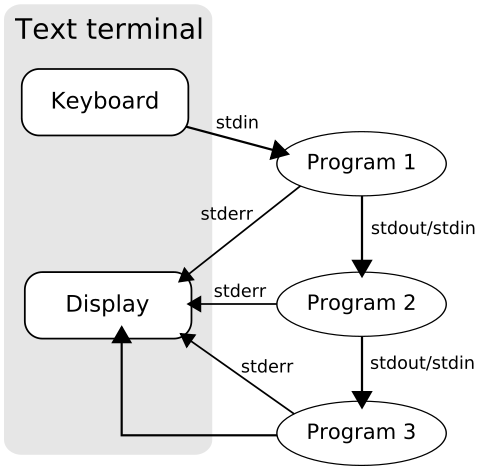
\includegraphics[scale=0.65,angle=-90]{pics/pipeline.eps} \\
\verb+http://is.gd/vGHO9J+ \\
\end{center}



\subsection{Program Design}
\vspace*{\fill}
\Huge
\begin{center}
"Consistency underlies all principles of quality." Frederick P. Brooks, Jr
\end{center}
\Normalsize
\vspace*{\fill}


\subsection{Program Design}
\verb+https://en.wikipedia.org/wiki/Unix_philosophy+ \\

UNIX programs...
\begin{itemize}
	\item ...are simple
	\item ...follow the element of least surprise
	\item ...accept input from {\tt stdin}
	\item ...generate output to {\tt stdout}
	\item ...generate meaningful error messages to {\tt stderr}
	\item ...have meaningful exit codes
	\item ...have a manual page
\end{itemize}
\subsection{Boot/Login process}
\small
\begin{verbatim}
[...]
total memory = 768 MB
avail memory = 732 MB
timecounter: Timecounters tick every 10.000 msec
mainbus0 (root)
[...]
boot device: xbd3
root on xbd3a dumps on xbd3b
mountroot: trying lfs...
mountroot: trying ffs...
root file system type: ffs
init: copying out path `/sbin/init' 11
[...]
Starting local daemons:.
Starting sendmail.
Starting sshd.
Starting snmpd.
Starting cron.

NetBSD/amd64 (panix.netmeister.org) (console)

login:
\end{verbatim}
\Normalsize

\subsection{Boot/Login process}
\small
\begin{verbatim}
[...]
total memory = 768 MB
avail memory = 732 MB
timecounter: Timecounters tick every 10.000 msec
mainbus0 (root)
[...]
boot device: xbd3
root on xbd3a dumps on xbd3b
mountroot: trying lfs...
mountroot: trying ffs...
root file system type: ffs
init: copying out path `/sbin/init' 11
[...]
Starting local daemons:.
Starting sendmail.
Starting sshd.
Starting snmpd.
Starting cron.

NetBSD/amd64 (panix.netmeister.org) (console)

login: jschauma
Password:
\end{verbatim}
\Normalsize


\subsection{Boot/Login process}
\small
\begin{verbatim}
[...]
total memory = 768 MB
avail memory = 732 MB
timecounter: Timecounters tick every 10.000 msec
mainbus0 (root)
[...]
boot device: xbd3
root on xbd3a dumps on xbd3b
mountroot: trying lfs...
mountroot: trying ffs...
root file system type: ffs
init: copying out path `/sbin/init' 11
[...]
Starting local daemons:.
Starting sendmail.
Starting sshd.
Starting snmpd.
Starting cron.

NetBSD/amd64 (panix.netmeister.org) (console)

login: jschauma
Password:
Last login: Sat Sep 10 14:27:56 2011 on console
Copyright (c) 1982, 1986, 1989, 1991, 1993
    The Regents of the University of California.  All rights reserved.

NetBSD 5.0.2 (PANIX-VC) #2: Tue Oct 19 16:30:57 EDT 2010

Welcome to NetBSD!

$
\end{verbatim}
\Normalsize

\subsection{Soooo... what exactly is a "shell"?}
\vspace*{\fill}
\begin{verbatim}
$ wget http://www.cs.stevens.edu/~jschauma/631/simple-shell.c
$ more simple-shell.c
$ cc -Wall -o mysh simple-shell.c
$ ./mysh
$$ /bin/ls
[...]
$$ ^D
$
\end{verbatim}
\vspace*{\fill}


\subsection{Files and Directories}
\begin{itemize}
	\item The UNIX {\bf filesystem} is a tree structure, with all partitions
		mounted under the root (/). File names may consist of any
		character except / and NUL as pathnames are a sequence of
		zero or more filenames separated by /'s.
\end{itemize}

\subsection{Files and Directories}
\begin{itemize}
	\item The UNIX {\bf filesystem} is a tree structure, with all partitions
		mounted under the root (/). File names may consist of any
		character except / and NUL as pathnames are a sequence of
		zero or more filenames separated by /'s.
	\item Directories are special "files" that contain mappings
		between {\em inodes} and {\em filenames}, called directory
		entries.
\end{itemize}


\subsection{Files and Directories}
\begin{itemize}
	\item The UNIX {\bf filesystem} is a tree structure, with all partitions
		mounted under the root (/). File names may consist of any
		character except / and NUL as pathnames are a sequence of
		zero or more filenames separated by /'s.
	\item Directories are special "files" that contain mappings
		between {\em inodes} and {\em filenames}, called directory
		entries.
	\item All processes have a current working directory from which
		all relative paths are specified. (Absolute paths begin
		with a slash, relative paths do not.)
\end{itemize}

\subsection{Listing files in a directory}
\vspace*{\fill}
\begin{verbatim}
$ wget http://www.cs.stevens.edu/~jschauma/631/simple-ls.c
$ more simple-ls.c
$ cc -Wall -o myls simple-ls.c
$ ./myls .
[...]
$
\end{verbatim}
\vspace*{\fill}


\subsection{User Identification}
\begin{itemize}
	\item {\em User ID}s and {\em group ID}s are numeric values used to
		identify users on the system and grant permissions appropriate to them.
	\item {\em Group ID}s come in two types; {\em primary} and {\em secondary}.
\end{itemize}
\vspace{.25in}

\begin{verbatim}
$ id
\end{verbatim}

\subsection{Unix Time Values}
{\em Calendar time}: measured in seconds since the UNIX epoch (Jan
1, 00:00:00, 1970, GMT). Stored in a variable of type {\tt time\_t}.
\\

\begin{verbatim}
$ date +%s
\end{verbatim}

\begin{center}
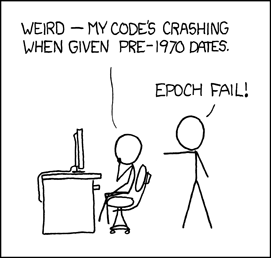
\includegraphics[scale=0.8,angle=-90]{pics/epoch-fail.eps} \\
\verb+https://www.xkcd.com/376/+ \\
\vspace{.25in}
\verb+https://en.wikipedia.org/wiki/Year_2038_problem+
\end{center}


\subsection{Unix Time Values}
{\em Process time}: central processor resources used by a process.
Measured in {\em clock ticks} ({\tt clock\_t}).  Three values:
\begin{itemize}
	\item clock time
	\item user CPU time
	\item system CPU time
\end{itemize}

\vspace*{\fill}
\begin{verbatim}
$ time grep -r _POSIX_SOURCE /usr/include >/dev/null
\end{verbatim}
\vspace*{\fill}

\subsection{Standard I/O}
\begin{itemize}
	\item	Standard I/O:
		\begin{itemize}
			\item {\bf file descriptors}: Small, non-negative
				integers which identify a file to the kernel.
				The shell can redirect any file descriptor.
			\item kernel provides {\bf unbuffered} I/O through e.g.
				{\tt open read write lseek close}
			\item kernel provides {\bf buffered} I/O through e.g.
				{\tt fopen fread fwrite getc putc}
		\end{itemize}
\end{itemize}
\vspace*{\fill}
\begin{verbatim}
$ wget http://www.cs.stevens.edu/~jschauma/631/simple-cat.c
$ wget http://www.cs.stevens.edu/~jschauma/631/simple-cat2.c
$ diff -bu simple-cat*.c
[...]
$
\end{verbatim}
\vspace*{\fill}


\subsection{Processes}
Programs executing in memory are called {\em processes}.
\begin{itemize}
	\item Programs are brought into memory via one of the
		six {\tt exec(3)} functions.  Each process is identified
		by a guaranteed unique non-negative integer called the
		{\em processes ID}. New processes can {\bf only} be
		created via the {\tt fork(2)} system call.
	\item {\bf process control} is performed mainly by the
		{\tt fork(2)}, {\tt exec(3)} and {\tt waitpid(2)} functions.
\end{itemize}
\vspace*{\fill}
\begin{verbatim}
$ wget http://www.cs.stevens.edu/~jschauma/631/pid.c
$ more pid.c
$ cc -Wall -o mypid pid.c
$ ./mypid .
[...]
$ echo $$
[...]
\end{verbatim}
\vspace*{\fill}

\subsection{Processes}
\vspace*{\fill}
\Huge
\begin{center}
	{\tt \$ pstree -hapun | more}
\end{center}
\Normalsize
\vspace*{\fill}



\subsection{Processes}
\small
\begin{verbatim}
[...]
total memory = 768 MB
avail memory = 732 MB
timecounter: Timecounters tick every 10.000 msec
mainbus0 (root)
[...]
boot device: xbd3
root on xbd3a dumps on xbd3b
mountroot: trying lfs...
mountroot: trying ffs...
root file system type: ffs
init: copying out path `/sbin/init' 11
[...]
Starting local daemons:.
Starting sendmail.
Starting sshd.
Starting snmpd.
Starting cron.

NetBSD/amd64 (panix.netmeister.org) (console)

login: jschauma
Password:
Last login: Sat Sep 10 14:27:56 2011 on console
Copyright (c) 1982, 1986, 1989, 1991, 1993
    The Regents of the University of California.  All rights reserved.

NetBSD 5.0.2 (PANIX-VC) #2: Tue Oct 19 16:30:57 EDT 2010

Welcome to NetBSD!

$
\end{verbatim}
\Normalsize



\subsection{Processes}
\begin{center}
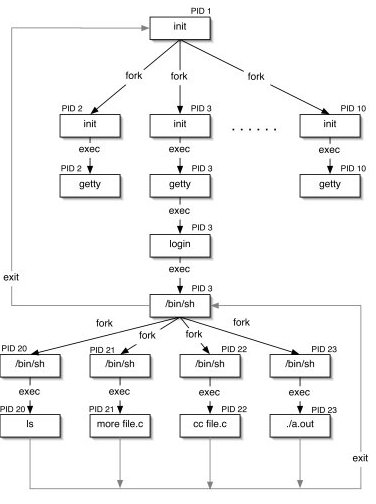
\includegraphics[scale=0.75]{pics/process-tree.eps} \\
\end{center}

\subsection{Signals}
\begin{itemize}
	\item	{\bf Signals} notify a {\em process} that a condition
			has occured. Signals may be
		\begin{itemize}
			\item ignored
			\item allowed to cause the default action
			\item caught and control transferred to a user defined function
		\end{itemize}
\end{itemize}
\vspace*{\fill}
\begin{center}
\begin{verbatim}
$ wget http://www.cs.stevens.edu/~jschauma/631/simple-shell2.c
$ more simple-shell2.c
$ cc -Wall -o mysh simple-shell2.c
$ ./mysh
$$ /bin/ls
[...]
$$ ^C
Caught SIGINT!
\end{verbatim}
\end{center}
\vspace*{\fill}

\subsection{Homework}
\begin{itemize}
	\item read {\tt intro(2)}, Stevens 1 \& 2
	\item follow, test and understand all examples from this lecture
	\item ask questions on the course mailing list and IRC channel
	\item bookmark these websites:
		\begin{itemize}
			\item {\tt https://www.cs.stevens.edu/\~{}jschauma/631/}
			\item {\tt http://pubs.opengroup.org/onlinepubs/9699919799/}
		\end{itemize}
%	\item get the full sources to NetBSD: \\
%		{\tt ftp://ftp.netbsd.org/pub/NetBSD/NetBSD-5.1/source/sets/}
	\item ensure you have an account on {\tt linux-lab.cs.stevens.edu}; see \\
		{\tt https://www.cs.stevens.edu/\~{}jschauma/631/linux-lab.html}
	\vspace{.5in}
	\item {\tt http://www.cs.stevens.edu/\~{}jschauma/631/intro.html}
	\item {\tt http://www.cs.stevens.edu/\~{}jschauma/631/f15-hw1.html}
\end{itemize}
\end{document}
